\receta{Marranitas}

Rinde 18 Unidades.

\begin{ingredientes}
\item 9 Plátanos Maduros
\item 1.5 kg Tocino
\item 1 L Aceite 
\item Agua
\item Bolsa plástica
\end{ingredientes}
\preparacion

Se cortan el tocino en cubos pequeños y se fritan para obtener chicharrones. Por aparte se pelan los plátanos y se cortan a la mitad de forma que salgan 2 troncos por plátano los cuales se fríen hasta que queden ligeramente dorados. .\\

Los troncos se pisan hasta obtener un masa que permita armar arepitas de plátano que se se les pone abundante agua para que le masa sea maleable.\\

A las arepitas mojadas se le ponen cubitos de chicharrón encima y con la masa se encierran los chicharrones formando bolitas. Para ayudar al proceso de cerrado se una una bolsa plástica para ayudar a mantener la forma de bola sin que se desbarate la masa.\\

Las bolitas se ponen a freir nuevamente hasta que queden doradas y se retiran rápidamente del aceite mientras este bien caliente para que no absorban mas grasa.\\
\clearpage
\vspace*{5cm}
\begin{center}
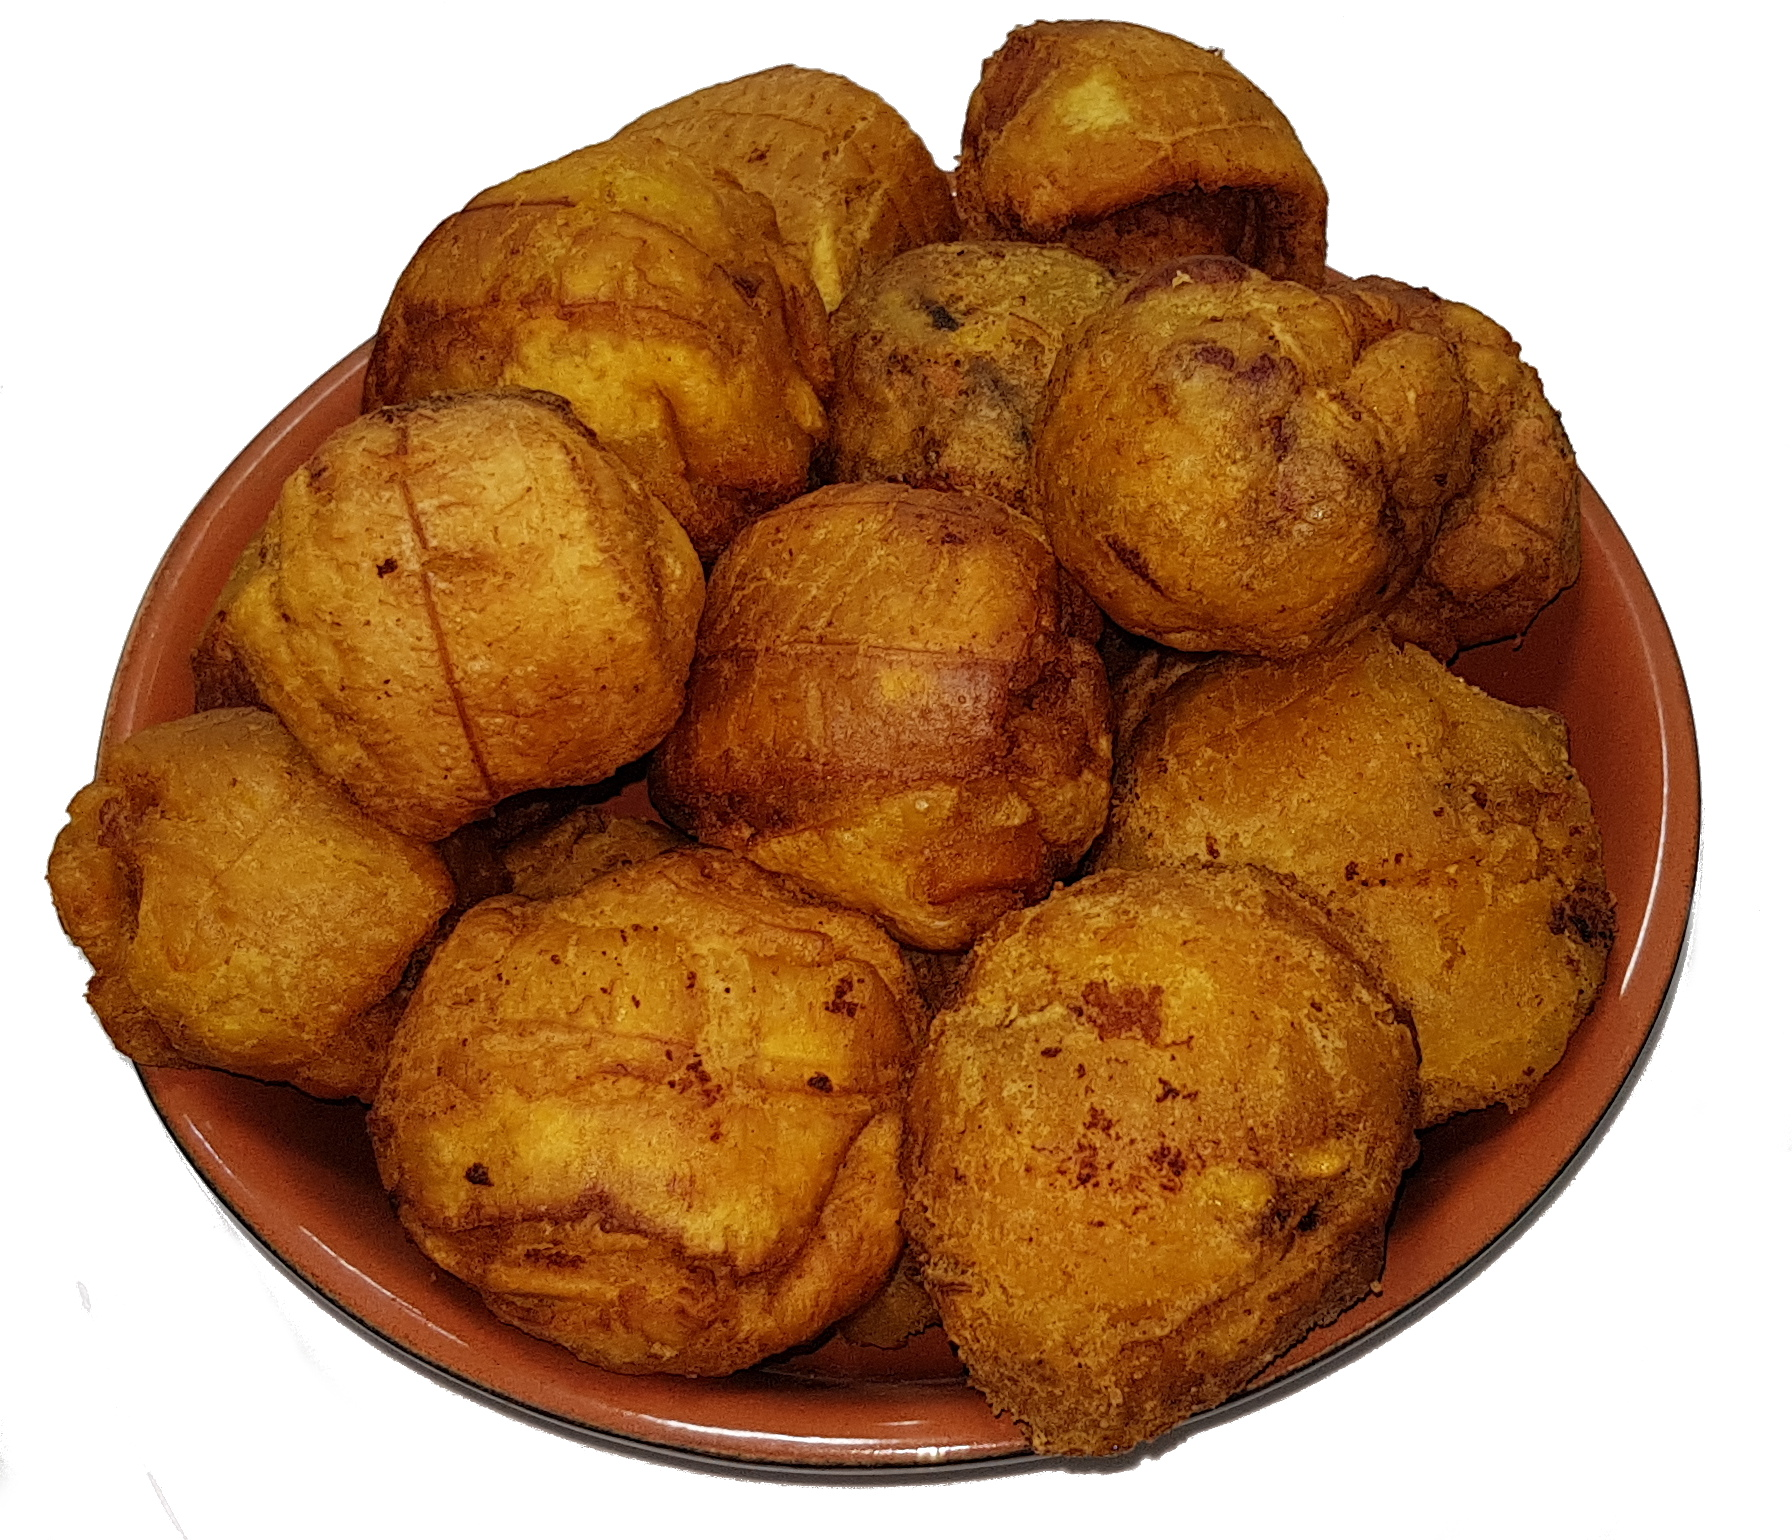
\includegraphics[width=0.8\textwidth]{fotos/marranitas}
\end{center}